% Copyright (C) Huawei Technologies Co., Ltd. 2024. All rights reserved.
% SPDX-License-Identifier: MIT

\begin{frame}{What can the industry do?}
    \begin{columns}[t]
        \column{.5\textwidth}{\uncover<1->{%
        \begin{center}
            %\hspace{-3mm}
            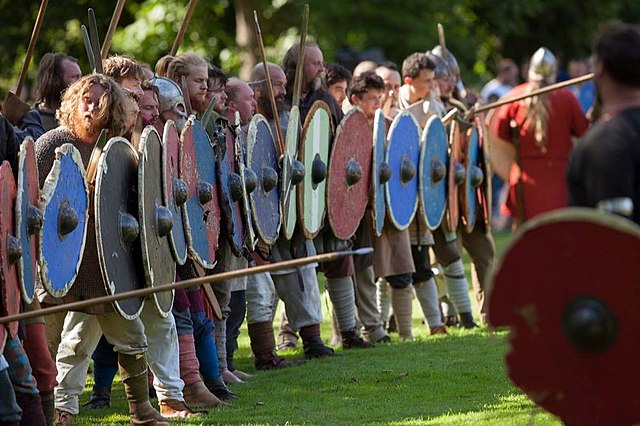
\includegraphics[trim=0 0 32mm 0, clip, width=40mm]{figs/shieldwall}
            \vspace{-4mm}
        \end{center}
        \begin{block}{Keep-it-simple and Overprotect?}
            \begin{itemize}\small\setlength\itemindent{-1em}\setlength\itemsep{1mm}
                \item Simplify design as much as possible
                \item Spray code with memory barriers and locks
                %The musl and MySQL projects conservatively overprotect the code by adding many strong barriers.
                %Depending on the hardware, the additional barriers may hurt performance.
                \item Risk: {\bf performance impact}
            \end{itemize}
        \end{block}}
        } \column{.5\textwidth} {\uncover<1->{%
        \begin{center}
            %\hspace{-3mm}
            
\includegraphics[trim=0 0 0 0, clip, width=40mm]{figs/witches}
            \vspace{-4mm}
        \end{center}
        \begin{block}{Rely on Expert Optimizations?}
            \begin{itemize}\small\setlength\itemindent{-1em}\setlength\itemsep{1mm}
                \item Exclusively rely on highly-skilled engineers
                \item Carefully design, implement and optimize
                \item Risk: {\bf error-prone, low maintainability}
            \end{itemize}
            %Over the course of 6 years, the Linux qspinlock was optimized by
            %highly-skilled engineers.
            %Still, one bug kept dormant during 12 releases.
        \end{block}}
        }
    \end{columns}
\end{frame}
